\documentclass[a4paper,12pt]{article}
\usepackage{graphicx}
\usepackage[UTF8]{ctex}

\graphicspath{{images/}}

\begin{document}
	\title{玩法介绍}
	\author{撰写人:朱善哲\\小组成员:马楷恒、王晟宇、李畅锦、朱博文}
	\date{2024年9月}
	\maketitle
	\section{界面UI}
		
		点击已部署单位会出现图1这四栏,点击“升级”会出现图2,点击“查看”会出现图3,点击“技能”可以使用“主动触发”技能,点击撤退则直接撤退。点击“升级”与“查看”弹出窗口后对局会时间暂停
	\section{玩法}
		点击待部署区单位后显示可部署地块,然后拖动到某个地块,相应地块出现图4,通过拖动方向来决定部署后朝向。可以通过消耗费用来进行升级,初始我方单位第一次升级可以选择分化成不同分支,之后升级仅进行数值上的加强。部署我方单位需要消耗费用。费用一般会自然回复,另外可以通过我方干员技能获取与歼灭某些敌方单位获取。
	\begin{figure}[p]
		\centering
		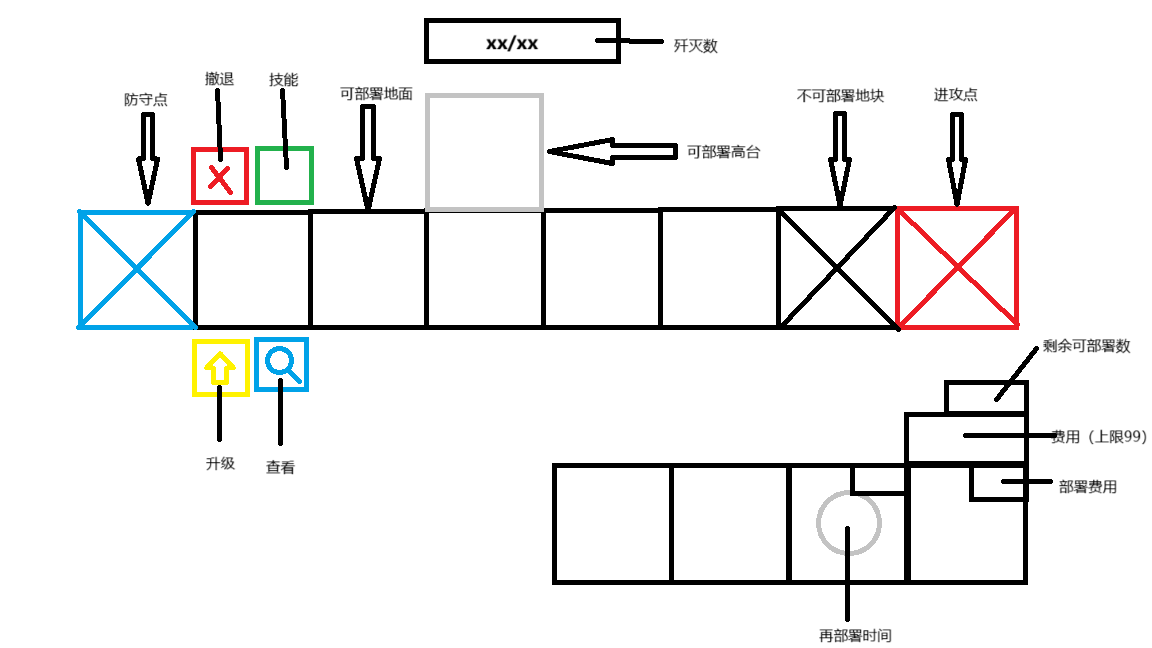
\includegraphics[width=1\textwidth]{map_intro}
		\caption{Map}
	\end{figure}
	\begin{figure}[p]
		\centering
		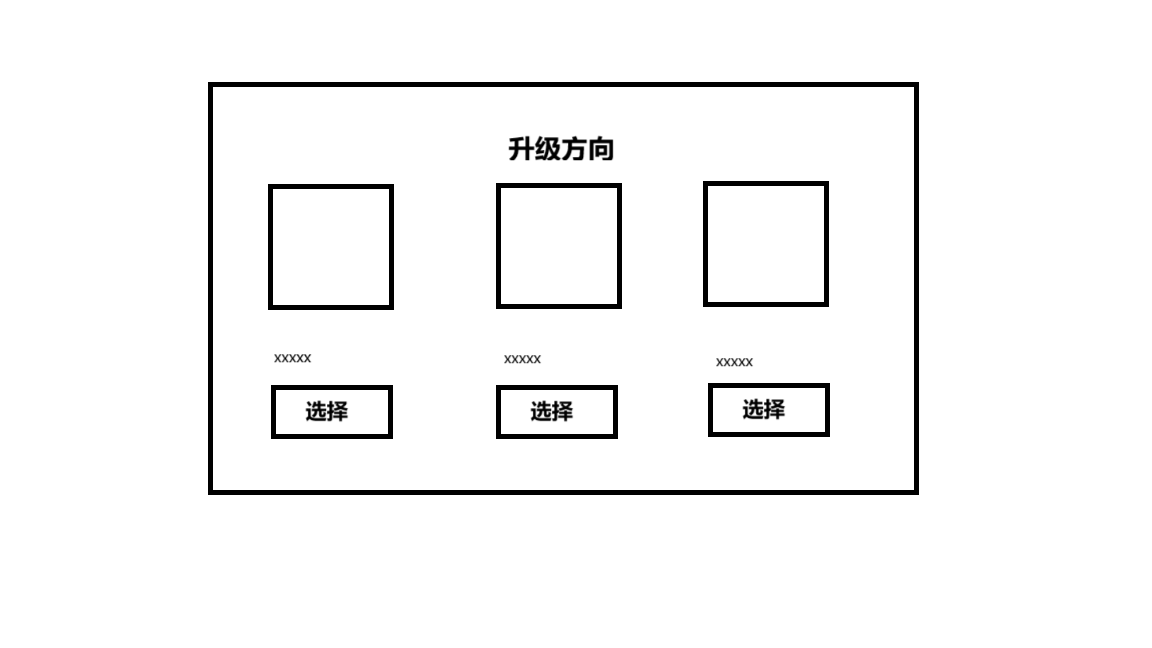
\includegraphics[width=1\textwidth]{choose}
		\caption{Choose}
	\end{figure}
	\begin{figure}[p]
		\centering
		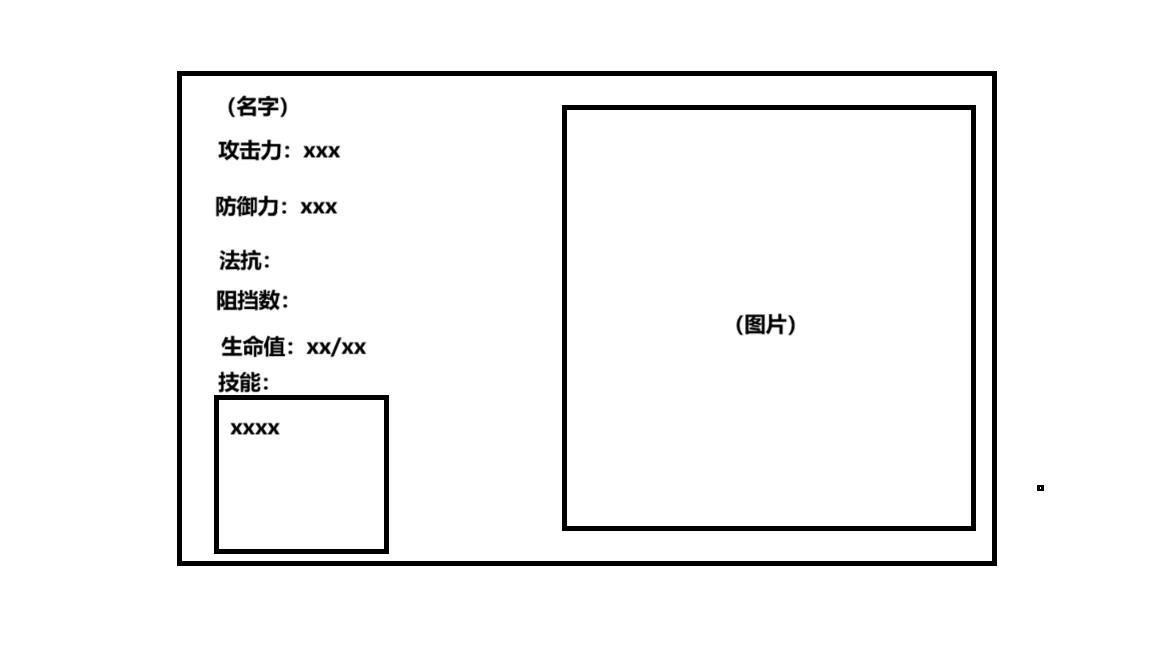
\includegraphics[width=1\textwidth]{look}
		\caption{Look}
	\end{figure}
	\begin{figure}[p]
		\centering
		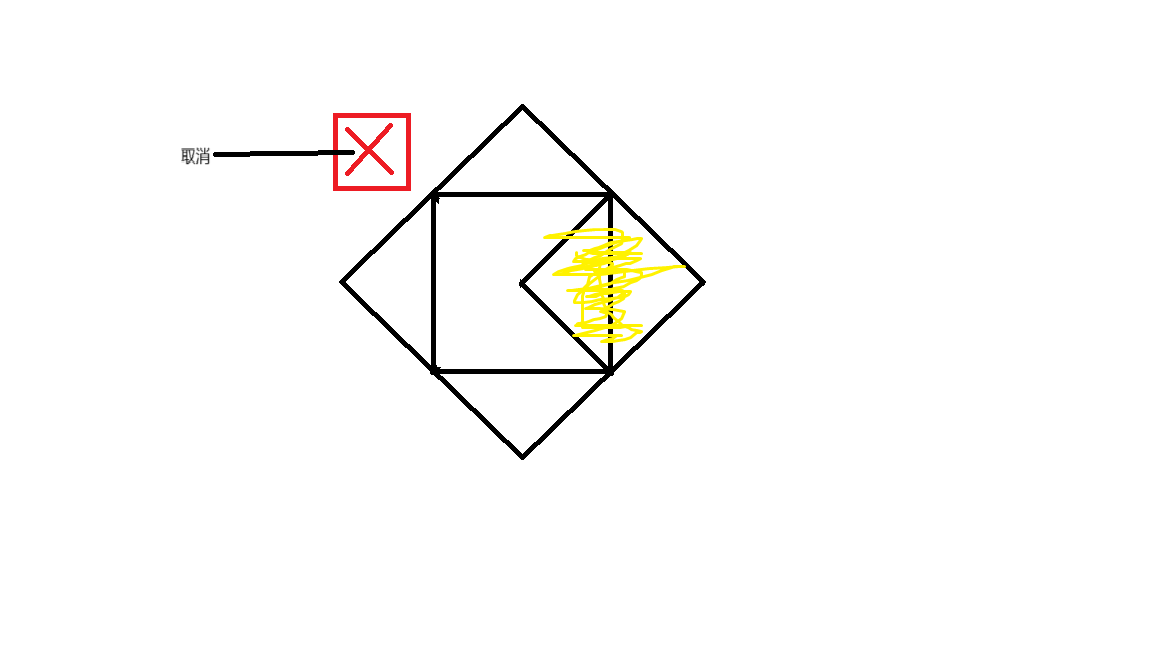
\includegraphics[width=1\textwidth]{put}
		\caption{Put}
	\end{figure}
\end{document}